\documentclass[pdftex,12pt,a4paper]{article}

\usepackage{graphicx}  
\usepackage[margin=2.5cm]{geometry}
\usepackage{breakcites}
\usepackage{indentfirst}
\usepackage{pgfgantt}
\usepackage{pdflscape}
\usepackage{float}
\usepackage{epsfig}
\usepackage{epstopdf}
\usepackage[cmex10]{amsmath}
\usepackage{stfloats}
\usepackage{multirow}

\renewcommand{\refname}{REFERENCES}
\linespread{1.3}

\usepackage{mathtools}
%\newcommand{\HRule}{\rule{\linewidth}{0.5mm}}
\thispagestyle{empty}
\begin{document}
\begin{titlepage}
\begin{center}
\textbf{}\\
\textbf{\Large{ISTANBUL TECHNICAL UNIVERSITY}}\\
\vspace{0.5cm}
\textbf{\Large{COMPUTER ENGINEERING DEPARTMENT}}\\
\vspace{2cm}
\textbf{\Large{BLG 242E\\ DIGITAL CIRCUITS LABORATORY\\ EXPERIMENT REPORT}}\\
\vspace{2.8cm}
\begin{table}[ht]
\centering
\Large{
\begin{tabular}{lcl}
\textbf{EXPERIMENT NO}  & : & 4 \\
\textbf{EXPERIMENT DATE}  & : & 22.04.2022 \\
\textbf{LAB SESSION}  & : & FRIDAY - 10.30 \\
\textbf{GROUP NO}  & : & 22 \\
\end{tabular}}
\end{table}
\vspace{1cm}
\textbf{\Large{GROUP MEMBERS:}}\\
\begin{table}[ht]
\centering
\Large{
\begin{tabular}{rcl}
150200056  & : & Furkan Salık\\
\end{tabular}}
\end{table}
\vspace{2.8cm}
\textbf{\Large{SPRING 2022}}

\end{center}

\end{titlepage}

\thispagestyle{empty}
\addtocontents{toc}{\contentsline {section}{\numberline {}FRONT COVER}{}}
\addtocontents{toc}{\contentsline {section}{\numberline {}CONTENTS}{}}
\setcounter{tocdepth}{4}
\tableofcontents
\clearpage

\setcounter{page}{1}

\section{INTRODUCTION [10 points]}

\begin{itemize}
    \item Implementation and usage of memory elements: latches and flip-flops.
    \item Establishing communication between circuit and oscillator.
\end{itemize}

\section{MATERIALS AND METHODS [40 points]}

\subsection{Part 1 - SR latch using NOR gates (without enable)}
\begin{figure}[H]
	\centering
	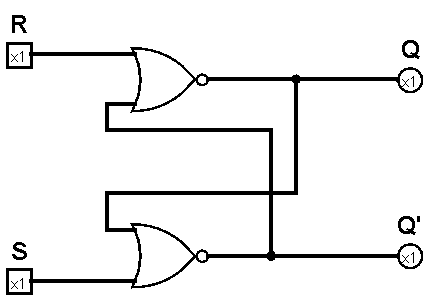
\includegraphics[width=0.7\textwidth]{circ1.png}	
	\caption{Circuit diagram.}
	\label{fig1}
\end{figure}

\begin{figure}[H]
	\centering
	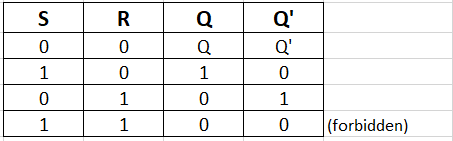
\includegraphics[width=0.7\textwidth]{truthtable1.PNG}	
	\caption{Truth table.}
	\label{fig1}
\end{figure}
Characteristic equation derived from the truth table is, \(Q(t+1) = S + Q(t) \cdot R'\)

\subsection{Part 2 - SR latch using NAND gates (with enable)}
\begin{figure}[H]
	\centering
	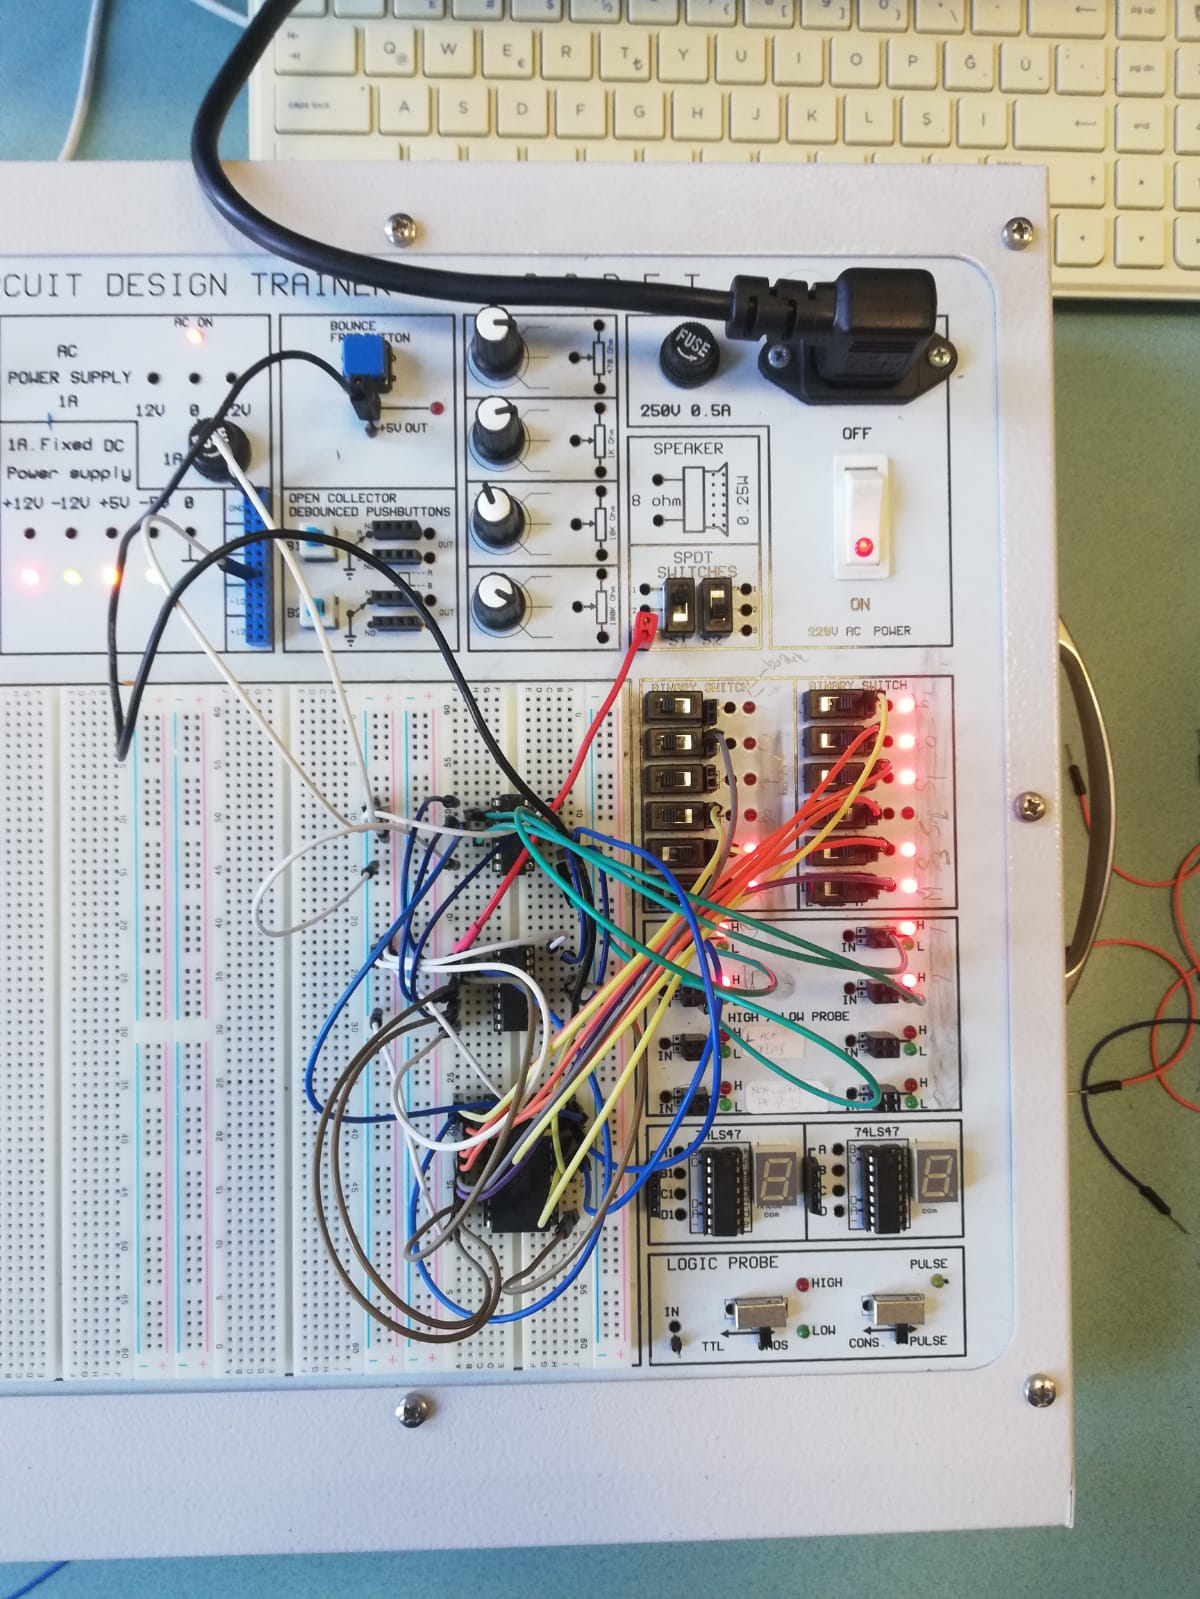
\includegraphics[width=0.7\textwidth]{circ2.PNG}	
	\caption{Circuit diagram.}
	\label{fig1}
\end{figure}

\begin{figure}[H]
	\centering
	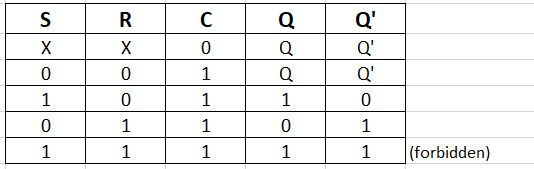
\includegraphics[width=0.7\textwidth]{truthtable2.PNG}	
	\caption{Truth table.}
	\label{fig1}
\end{figure}

Characteristic equation derived from the truth table is, \(Q(t+1) = S \cdot E + Q(t) \cdot R' \cdot E + Q(t) \cdot E'\)

\subsection{Part 3 - Negative edge triggered D flip-flop}
\begin{figure}[H]
	\centering
	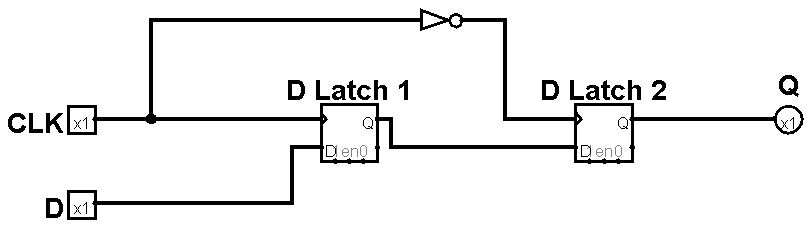
\includegraphics[width=0.7\textwidth]{circ3.PNG}	
	\caption{Circuit diagram.}
	\label{fig1}
\end{figure}

\begin{figure}[H]
	\centering
	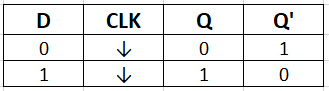
\includegraphics[width=0.5\textwidth]{truthtable3.PNG}	
	\caption{Truth table.}
	\label{fig1}
\end{figure}

\subsection{Part 5 - Counter (0-5 range)}
\begin{figure}[H]
	\centering
	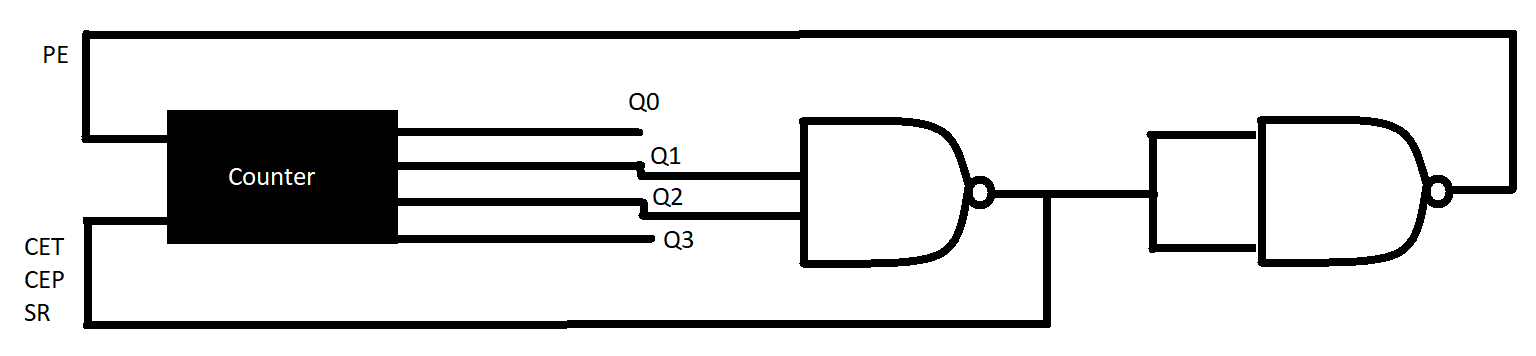
\includegraphics[width=1\textwidth]{circ5.PNG}	
	\caption{Circuit diagram.}
	\label{fig1}
\end{figure}
This circuit works as, if the current number is not 6 (by \(Q_1\) NAND \(Q_2\), since  6 = 0110), CET, CEP and SR inputs of the counter (74xx161 IC) is set to 1, and if the current number is 6, (the second NAND gate behaves as if it is a NOT gate) PE input of the counter is set to 1. This design is prepared according to the datasheet of the counter.

\section{RESULTS [15 points]}
First, I have implemented an SR latch using NOR gates, which did not have an enable input. Then, an SR latch using NAND gates, with an enable input is implemented. Thirdly, a negative edge-trigger is realized using 2 latches. In the fourth part, a pulse generator is made, several inputs are given and signals are seen from oscillator. In the last part, a counter that ranges between [0-5] is implemented. Its outputs were seen in display part of CADET.

\section{DISCUSSION [25 points]}
Part 1 and part 2 are implemented using feedback connections, which is the idea behind creating memory cells. In those parts, the first thing catching my attention was the difference between forbidden outputs, the difference stems from the introduction of enable input to NAND gates. In part 3, negative edge triggered flip-flop is implemented, 2 latches were needed for this, as it can be seen from the circuit diagram. This structure is also known as master/slave flip-flop. In part 4, circular shift register was used, several inputs were given, and outputs with different frequencies were obtained from the oscillator. In the last part, a counter that ranges in [0-5] is implemented. This is accomplished as resetting the counter if the number has been 6, incrementing otherwise.

\section{CONCLUSION [10 points]}
In the fourth part, there was a confusion, since there were so many connections to be made, and oscillator had to be used. Also, giving correct inputs for getting correct frequency outputs was hard to do. I learned how to implement and use data storage elements, and how to make a connection between oscillator and circuit.

\newpage
\addcontentsline{toc}{section}{\numberline {}REFERENCES}

\bibliographystyle{unsrt}
\bibliography{reference}

\end{document}

